\subsection{Approach}
\label{sec:soft_cut_approach}

For the soft cut detection we decided to use a deep learning approach.
More concrete we used the RNN/LSTM implementation by Jeff Donahue\footnote{\url{https://github.com/BVLC/caffe/pull/2033}}. \\
This RNN/LSTM implementation takes two different inputs: On the one hand the raw pixel values and on the other hand a tagging sequence.
A tagging sequence represents sequences of frames, where one sequence of frames might represent a soft cut in our case.
Using this implementation allows us to incorporate the information of a frame, which is at the beginning of a frame sequence, to a frame, which is located later in the same sequence.
So the net memorizes previous decision along a sequence of frames. \\
But using this architecture has one problem, as stated by Jeff Donahue: ``Backpropagation [through the LSTM] is truncated along the batch boundaries'' [TODO: Quelle].
So one or more frame sequences has to fit exactly into the batch size used by the RNN/LSTM.
This is hard to archive if we want to use variable length of frame sequences.
Therefore we decided to use a fixed size for the sequences of frames in a tagging sequence, i.e. we only check for example 10 consecutive frames of being a soft cut or not.  \\
However, we still want to find soft cut of arbitrary length in a video.
To achieve this, we repeatedly test fixed-size frame sequences.
In Figure~\ref{fig:soft_cut_approach} an example is shown.
\begin{figure}[!htb]
	\centering
	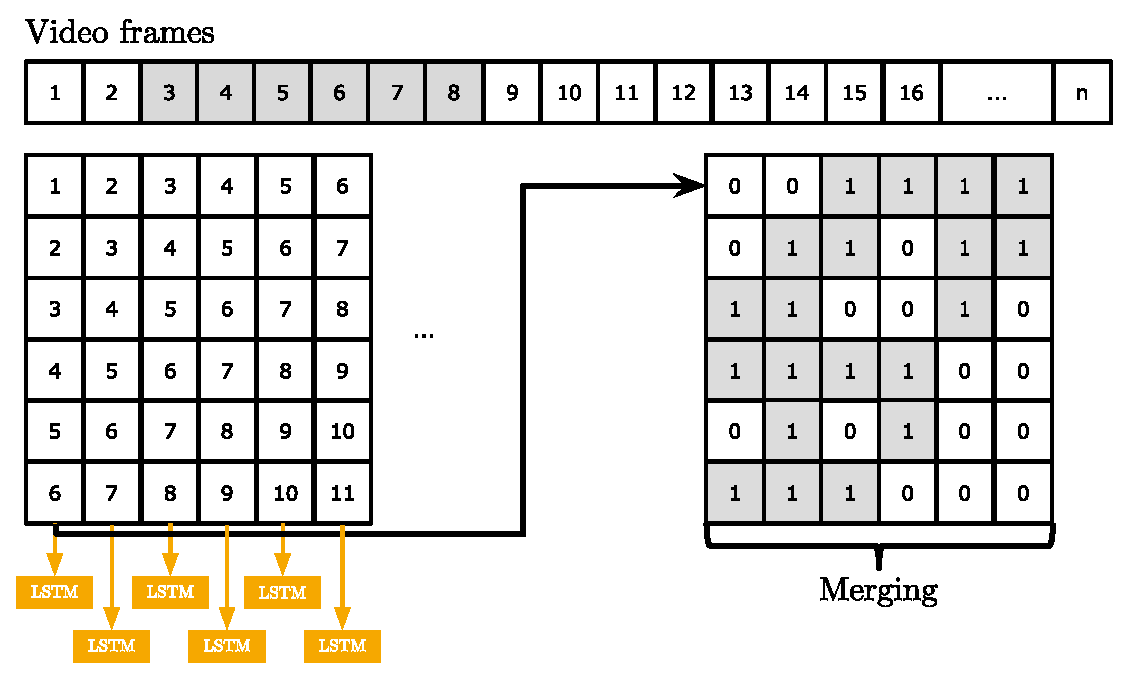
\includegraphics[scale=.7]{images/soft_cut_approach.eps}
	\caption{To classify soft cuts of arbitrary length, we repeatedly test fixed-size frame sequences. In this example we test sequences of size six. Afterwards the predictions given by the RNN/LSTM are merged, so that we have one prediction per frame.}
	\label{fig:soft_cut_approach}
\end{figure}
We have a video with \textit{n} frames.
The frames from three to eight represent a soft cut.
We now generated for each frame a frame sequence of size six.
Those sequences are then classified by the RNN/LSTM.
The output of the RNN/LSTM is zero, if a frame does not belong to a soft cut, and one, otherwise.
In the end we have up six prediction per frame, which have to be merged, so that we only have one prediction per frame.
After the merging step consecutive frames, which got a prediction of one, i.e. the frame is part of an soft cut, represent a soft cut. \\
In the following several strategies for combining the multiple frame prediction into one prediction are presented.
An overview over all strategies can be found in Figure~\ref{fig:merging_strategies}
\begin{figure}[!htb]
	\centering
	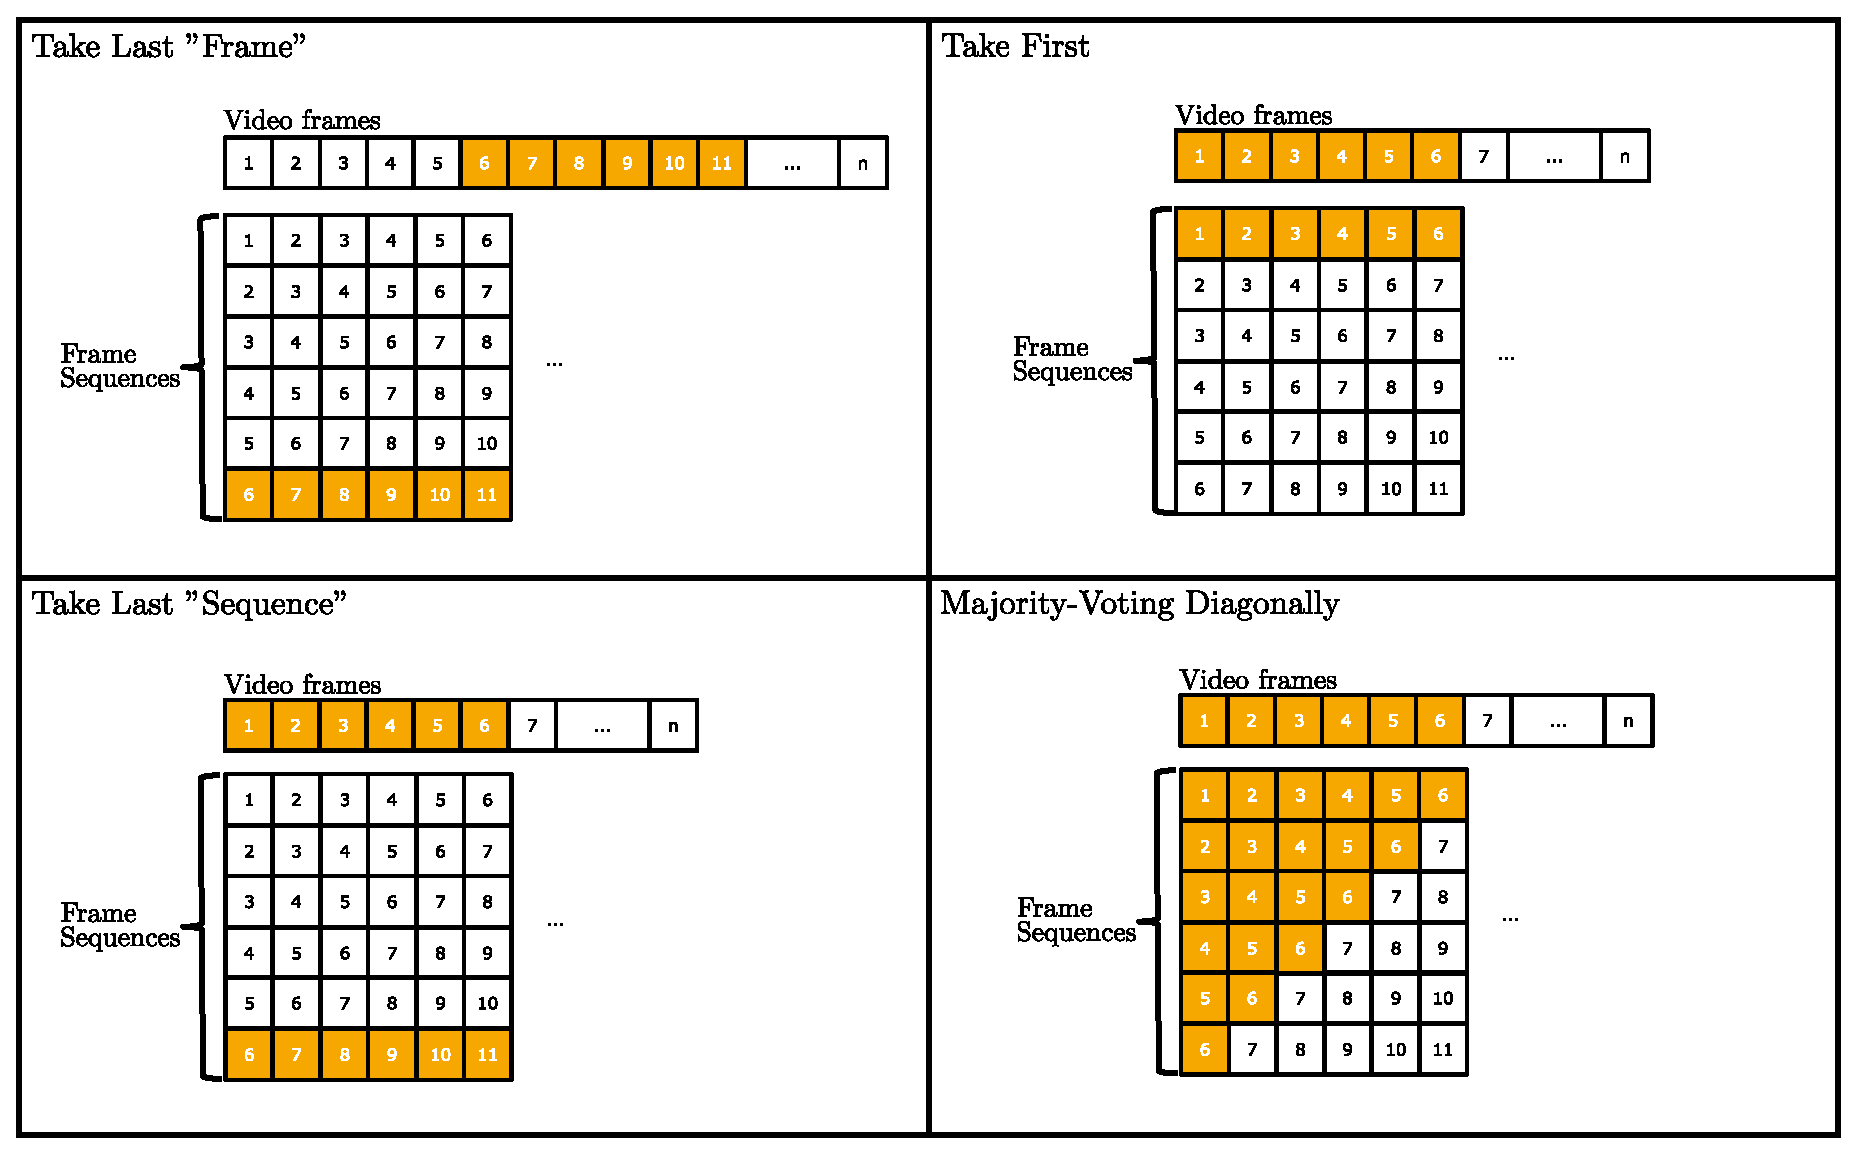
\includegraphics[scale=.5]{images/merging_strategies.eps}
	\caption{To merge the multiple predictions per frame into one, we implemented serval strategies: \textit{Take Last 'Frame'} (top left): The prediction of the frame, where the frame is the last of a frame sequence, is taken. \textit{Take Last 'Sequence'} (bottom left): The last prediction of the frame sequence belonging to a frame is taken. \textit{Take First} (top right): The first prediction of the frame sequence is taken. \textit{Majority-Voting Diagonally} (bottom right): The majority voting among all preditions of the frame is taken.}
	\label{fig:merging_strategies}
\end{figure}

\paragraph{Take First}
A first simple strategy is to take always the first prediction of a frame sequence.

\paragraph{Take Last 'Sequence'}
A second simple strategy is to take the last prediction of a frame sequence.
The intuition behind this is, that an RNN/LSTM becomes more and more certain after having seen multiple frames of the sequence.

\paragraph{Take Last 'Frame'}
In the \textit{Take Last 'Frame'} strategy, the prediction of the frame, where the frame is the last in the sequence, is taken.

\paragraph{Majority-Voting Diagonally}
Each frame is predicted up to \textit{x} times.
In our example it is up to six times.
In the \textit{Majority-Voting Diagonally} all of those predictions are taken and the majority voting among those is taken as prediction for the frame.


So far we explained how to detect soft cuts in general using a RNN/LSTM.
Now, the different architectures of the RNN/LSTM nets we used, are shown.


